\documentclass[adraft,creativecommons]{eptcs}
\usepackage[utf8]{inputenc}

\usepackage{underscore}

\usepackage[T1]{fontenc}
\usepackage{mathpartir}
\usepackage{amssymb}
\usepackage{amsmath}
\usepackage{amsthm}
\usepackage{braket}
\usepackage{xspace}
\usepackage[capitalize]{cleveref}
\crefformat{section}{\S#2#1#3}
\crefformat{lstlisting}{Listing #2#1#3}
\crefmultiformat{lstlisting}{Listings~#2#1#3}%
{ and~#2#1#3}{, #2#1#3}{ and~#2#1#3}
\crefrangeformat{lstlisting}{Listings~#3#1#4--#5#2#6}

% \usepackage{adjustbox}
\usepackage{tikz}
\usetikzlibrary{quantikz}

% From: https://tomhennigan.blogspot.com/2012/01/grouped-emails-in-latex-with-href-and.html
\newcommand{\mailtodomain}[1]{\href{mailto:#1}{\nolinkurl{#1}}}

\usepackage{xcolor}
\definecolor{dkgreen}{rgb}{0,0.35,0}

\usepackage{listings}
\lstloadlanguages{Haskell}
\lstdefinelanguage{QHaskell}{
    language     = Haskell,
    morekeywords = {bit, qbit, vector, complex, unit, U, C, meas, apply, to, requires, ensures},
}

\lstset{
    basicstyle=\small\ttfamily,
    captionpos=b,
    numbers=left,
    numberstyle=\tiny\color{gray},
    flexiblecolumns=false,
    basewidth={0.5em,0.5em},
    commentstyle=\color{dkgreen},
    keywordstyle=\bfseries\color{blue},
    stringstyle=\color{violet},
    literate=
        {√}{{$\surd$}}1
        {⇐}{{$\Leftarrow$}}1 {⇒}{{$\Rightarrow$}}2
        {->}{{$\rightarrow$}}2 {<-}{{$\leftarrow$}}2
        {|}{{$\vert$}}1 {⟩}{{$\rangle$}}1
        {∧}{{$\wedge$}}1 {∨}{{$\vee$}}1
        {∈}{{$\in$}}1 {Π}{{$\Pi$}}2
        {\\}{{$\lambda$}}1
        {∃}{{$\exists$}}2 {∀}{{$\forall$}}2
        {⊗}{{$\otimes$}}2 {⊕}{{$\oplus$}}2
        {⊤}{{$\top$}}2
        {=q}{{$=_q$}}2 {=c}{{$=_c$}}2
        {_1}{{$_1$}}1 {_2}{{$_2$}}1
        {α}{{$\alpha$}}1 {β}{{$\beta$}}1
        {ψ}{{$\psi$}}1
        {_i}{{$_i$}}1 {_x}{{$_x$}}1 {_y}{{$_y$}}1
        {\ .\ }{{$\cdot$}}1
        {β00}{{$\beta_{00}$}}2
        {==}{{$=$}}1 {!=}{{$\neq$}}1
}

\newcommand{\HoareT}[3]{
    \{#1\} ~#2~ \{#3\}
}

\theoremstyle{definition}
\newtheorem{definition}{Definition}[section]
\theoremstyle{remark}
\newtheorem*{remark}{Remark}

% \usepackage{blindtext}
\usepackage{ottalt}
\inputott{htt.ott.tex}

\def\titlerunning{Quantum Hoare Type Theory}
\def\authorrunning{Kartik Singhal}

\hypersetup{
    pdftitle={\titlerunning},
    pdfsubject={Computer Science},
    pdfauthor={\authorrunning},
    pdfkeywords={General programming languages, Quantum computation, Functional languages, Program specifications, Pre- and post-conditions, Type theory, Hoare logic}
}

\title{\titlerunning}

\author{
\authorrunning
\institute{University of Chicago}
\email{\mailtodomain{ks@cs.uchicago.edu}}
}

\begin{document}

\maketitle

\begin{abstract}
    As quantum computers become real, it is high time we come up with effective techniques that help programmers write correct quantum programs. In classical computing, formal verification and sound static type systems prevent several classes of bugs from being introduced. There is a need for similar techniques in the quantum regime. Inspired by Hoare Type Theory in the classical paradigm, we propose Quantum Hoare Types by extending the Quantum IO Monad by indexing it with pre- and postconditions that serve as program specifications. In this paper, we introduce Quantum Hoare Type Theory (QHTT), present its syntax and typing rules, and demonstrate its effectiveness with the help of examples.

    QHTT has the potential to be a unified system for programming, specifying, and reasoning about quantum programs.
\end{abstract}

\thispagestyle{empty}

\tableofcontents

\listoftables

\listoffigures

\lstlistoflistings

\setlength{\parskip}{1em}

\section{Introduction}

Quantum computation is fast becoming a reality over the last couple of years with the advent of real machines as recent breakthroughs such as Google's recent demonstration of the so called ``quantum supremacy'' shows. With advances in hardware, there is similar acceleration in the development of software for quantum machines which in turn requires development of special-purpose programming languages. Several efforts in this direction both from academia and industry have recently led to a number of programming languages aimed at quantum computing such as Q\#, Quipper, Scaffold, and Silq.

There is also a sudden need to prepare and train the upcoming generation of quantum programmers who sometimes have little to no previous exposure to the fundamental concepts in quantum computation. If we were to put ourselves in the position of a beginner to quantum programming, we may start by learning basic concepts such as what is a qubit, what does it mean for a qubit to be a superposition of 0 and 1, and the most perplexing of all: entanglement. We may then try to write some simple programs in a suitable quantum programming language to aid our understanding. We may even be able to run some of these programs on simulators and even on real machines. But we will make mistakes while writing these programs and sometimes those mistakes may be apparent from the output, a lot of the times (as a beginner) they may be not. What can we do?

A common method to test our assumptions while programming in the classical realm is to write assertions about what we believe to be the truth at a point in the program. These assertions are usually dynamic in nature, meaning they are only tested while running the program and involve a cycle of writing, running, debugging and rerunning the program. While this may be a suitable approach in classical computing, it is quite wasteful of the limited quantum resources if we were to apply it to quantum programming. Further, this approach is impossible to use if the number of qubits is just over 50 or so as we hit the limits of both current quantum machines and classical simulation. Yet, there have been a lot of recent proposals to use runtime assertions for debugging quantum programs.

What can we from the programming languages community offer that can help the upcoming workforce of quantum programers avoid mistakes in their programs?

In classical software development, the use of strong static type systems has been proven to be hugely beneficial in avoiding large classes of bugs before running the programs. Recent mainstream languages such as Rust even manage to statically prevent memory safety bugs that have been notorious for being the root causes of a large swath of security vulnerabilities found in production software written in unsafe languages such as C. There is a similar need for innovation in type systems for quantum programming languages.

Recent academic languages such as QWire and Silq that employ a linear type system to statically enforce the no-cloning theorem of quantum mechanics show promise in the validity of statically preventing bugs in the quantum domain. However, semantic properties about the quantum state such as whether a qubit is in superposition or whether it is entangled with some other qubit have not been tackled with the help of types. Further, assertions in the form of pre- and postconditions around small pieces of code have shown the most promise in the quantum domain. It seems fair as we humans can only hold so much information about the quantum state in our brains that it makes sense to be able to reason about pieces of quantum code in a modular manner.

The most common approach to reason with pre- and postconditions in the classical domain is to use variations of Floyd-Hoare logic that utilize specification triples of the form $\HoareT{P}{c}{Q}$, where $c$ is the program to be executed, $P$ a proposition on the initial state associated with the program (precondition) and, $Q$ that on the final state (postcondition). The intuitive reading of such as triple is that if the precondition holds true on the program state before executing the program, then if the program terminates, the postcondition must hold true. These triples along with a set of axioms and inference rules for composing them together have proven to be quite effective in proving correctness of classical state-manipulating (imperative) programs over the last several decades. It is no surprise that similar logics have appeared in the quantum computing domain as well.

Hoare Type Theory (HTT) incorporates Hoare-style specifications into types that can then be used to statically enforce desired properties about the program state. This is made possible with the use of dependent types that can depend on values (instead of just other types) and add immense expressive power to a programming language. In effect, we obtain a functional programming language in which imperative code is encapsulated within a computation type which is indexed by the type of the result of the computation, and its specification in the form of pre- and postconditions. We then obtain a system where the process of type checking a program becomes equivalent to verifying that the program meets the given specification. In this work, we consider the problem of reasoning about quantum programs in HTT and present our Quantum Hoare Type Theory (QHTT).

To achieve this, we replace the classical primitive commands from the original HTT with quantum-specific primitive commands and make use of a novel approach by Unruh \cite{unruh2019} and employ ghost variables for reasoning locally about quantum state in our quantum proposition logic. Further, the use of ghost variables enables an expressive language of propositions in which we can specify predicates about the equality, superposition and entanglement of qubits.

We limit our presentation to quantum programs that do not involve iteration. This is not to suggest that iteration is not supported in the system, only that we are yet to study it.

Our investigation suggests that QHTT has the potential to be a unified system for programming, specifying, and reasoning about quantum programs.

\section{Background}
In this section, we provide background on the core ideas from existing literature that form the foundation for our work --- Hoare logic, Hoare Type Theory (HTT), quantum computation, and quantum Hoare logic defined with ghost variables.

\subsection{Floyd-Hoare logic}
In the late 1960's, Robert Floyd and Tony Hoare came up with a set of axioms and rules of inference that can be used to prove properties of computer programs. This approach is commonly just known as Hoare logic as Hoare was the first to apply it to text-based programs, while Floyd had applied it to flowcharts. Here we present the axioms and rules of Hoare logic in a natural deduction style.

As noted above, this technique involves the use of Hoare triples of the form:
\begin{mathpar}
    \HoareT{P}{c}{Q}
\end{mathpar}
which can be interpreted as ``if the precondition $P$ is true before the execution of the program $c$, then the postcondition $Q$ will be true on its completion.''

In the classical setting, the most important command is an assignment statement. Hoare logic states the following axiom for assignment:
\begin{mathpar}
    \inferrule[Axiom of Assignment]
    {}
    {\HoareT{P[x \rightarrow e]}{x := e}{P}}
\end{mathpar}
where $x$ is an assignable (variable) and $e$ is an expression. The meaning of this fact is that the precondition is obtained from the postcondition $P$ by substituting $e$ for all free occurrences of $x$ in $P$.

Further, there are rules of inference that are required to derive new theorems from one or more axioms or theorems already proved. We first look at the two ``rules of consequence'':
\begin{mathpar}
    \inferrule[Weakening the postcondition]
    {\HoareT{P}{c}{Q} \\ Q \Rightarrow R}
    {\HoareT{P}{c}{R}}

    \inferrule[Strengthening the precondition]
    {P \Rightarrow Q \\ \HoareT{Q}{c}{R}}
    {\HoareT{P}{c}{R}}
\end{mathpar}

The first rule says that if the execution of a program $c$ ensures the truth of postcondition $Q$, then it also ensures the truth of any proposition $R$ logically implied by $Q$. This effectively lets us weaken the postcondition.

In the other direction, we can strengthen the precondition using the second rule which says that if $Q$ is a precondition of program $c$, then so is any other proposition $P$ that logically implies $Q$.

Alternatively, we can provide a single rule combining the two above:
\begin{mathpar}
    \inferrule[Rule of consequence]
    {P \Rightarrow Q \\ \HoareT{Q}{c}{R} \\ R \Rightarrow S}
    {\HoareT{P}{c}{S}}
\end{mathpar}

The next rule lets us compose sequential programs together:
\begin{mathpar}
    \inferrule[Rule of Composition]
    {\HoareT{P}{c}{Q} \\ \HoareT{Q}{d}{R}}
    {\HoareT{P}{c\ \textbf{;}\ d}{R}}
\end{mathpar}
where semicolon denotes sequential composition of programs. The rule of composition states that if the postcondition of the first program is identical to the precondition of the second program under which it satisfies its postcondition $R$, then the composition of the programs will satisfy $R$, given that the first program satisfies its precondition $P$.

These are the most important rules that we will need to understand the formal system presented below. We do not present other rules such as that for iteration (which we will not need) and others that can be derived. We also note that since we do not have an iteration construct in our system, we do not run into the issue of reasoning about termination of programs. In other words, all programs presented in our system will be terminating.

There is one other crucial concept we need to understand before moving to the next section. Let us motivate it with the help of an example that will also serve the purpose of demonstrating how to use Hoare logic. Suppose we are given the following simple triple:
\begin{mathpar}
    \HoareT{x = 1}{x := 5}{x > 0}
\end{mathpar}

This obviously seems correct. But how can we mechanically use the formal system just described to show this triple is valid? The missing piece is the idea of a ``strongest postcondition''. Given the assignment statement, we can compute the strongest possible postcondition to be $x = 5$, which implies $x > 0$ that is the given postcondition. Now, we can use the first rule of consequence (weakening the postcondition) to derive the given triple. We will use the notation $sp(c, P)$ for the function that computes the strongest postcondition for a given statement $c$ and precondition $P$.

In Hoare Type Theory that we describe next and its quantum variant later, inferring the strongest postcondition for each statement will be the most important step during the process of type checking.

\subsection{Hoare Type Theory}

A type theory is a formal system of rewriting in which each term has a type, notated as $t:A$ for a term $t$ and a type $A$. A type theory that admits dependent types can be called a dependent type theory. Dependent type theories can be viewed as logical systems as popularized by the Curry-Howard correspondence (also known as the principle of propositions-as-types or of proofs-as-programs). Under this interpretation, logical quantifiers such as $\forall$ (universal) and $\exists$ (existential) correspond respectively to the dependent product ($\Pi$) and sum ($\Sigma$) type in the type theory, for example. It turns out that with the expressive power that comes with dependent types, it becomes possible to encode behavioral specifications of programs as their types which can be viewed as theorems. To prove the theorem corresponds to writing a program of that type and checking the proof translates to type checking.

Hoare Type Theory or HTT is a specific dependent type theory that introduces a type constructor called a ``Hoare type'' which both isolates effectful programs from the remaining functional core language and lets us specify their behavior. In its most basic form, a Hoare type is written as:
\begin{mathpar}
    \HoareT{P}{x:A}{Q}
\end{mathpar}
where $P$ and $Q$ are pre- and postconditions and $x:A$ is the return value, thus incorporating the specification methodology of Hoare logic into types. Hoare types can also be seen as ``monads'' that are common in functional programming and are similarly used to isolate effects. The main difference is that such a ``Hoare monad'' is not only indexed by the the type of computation but also with the pre- and postconditions that must be satisfied by the given computation.

How do we verify programs in HTT? Like we saw above in the example for Hoare logic, a user can provide arbitrary pre- and postconditions as the type for their program. In HTT, the process of verifying that the given triple is valid is performed during type checking. In order to do so, the type checking process in HTT is carefully divided into two phases: The first phase performs basic type checking and infers the strongest postconditions in the form of verification conditions at each step of the program. In the second phase, we need to verify that the verification conditions hold. The first phase is decidable but the second phase may not be, hence for the second phase, either the verification conditions are deferred to an automated theorem prover (such as Z3) or need to be validated manually (in an interactive theorem prover such as Coq).

Let's consider the example we saw in the previous section written in HTT:\medskip\\
\indent\indent\lstinline[language=QHaskell]!x := 5 : {x = 1} r:unit {x > 0}!
\medskip\\where $r$ is the variable that holds the result of the assignment statement. Since an assignment returns nothing, we see the type of output is $unit$ and the pre- and postconditions are same as before.

In an alternate syntax inspired by the F* programming language (which takes a hybrid approach between automated and interactive theorem proving and is an evolution of HTT), that we will use in our presentation in this work, we can write the above triple as:\medskip\\
\indent\indent\lstinline[language=QHaskell]!x := 5 : ST r:unit (requires {x = 1}) (ensures {x > 0})!
\medskip\\which may be clearer to people familiar with Haskell. Here, $ST$ is the state monad that encapsulates computations that modify state (here assignment) and it is indexed by the result of the computation and its two pre- and postconditions. The keywords $requires$ and $ensures$ provide extra clarity for people unfamiliar with Hoare logic and explicitly naming the computational effect monad, $ST$, helps ensure multiple effects can be supported simultaneously. Inspired by this notation, we will christen our quantum state monad as $QST$. But let us first talk about quantum computation.

\subsection{Quantum Computation}
It is well known that quantum computation can be described in terms of elementary linear algebra. We assume familiarity with basic notions such as vectors, matrices, vector spaces, inner products, bases, linear independence, etc.

TODO: consider rewriting in terms of the four postulates of state space, dynamic evolution of closed systems, measurement and composite systems.

Quantum computation is usually described over a specific vector space called the \textit{Hilbert space}, $\mathcal{H}$, which for our purposes can be thought of as an $n$-dimensional complex vector space equipped with an inner product ($\mathbb{C}^n$). In this work, we will often use the term ``state space'' to refer to a finite dimensional Hilbert space.

The basic unit of information in quantum computation is a qubit, that can be represented using a unit vector in the two-dimensional complex vector space, $\mathbb{C}^2$. Using Dirac's bra-ket notation, we can write an arbitrary qubit, $\psi$, as a linear combination (or \textit{superposition}) of the computational basis vectors:
\begin{mathpar}
 \psi = \alpha\ket{0} + \beta\ket{1}
\end{mathpar}
where
\begin{mathpar}
\ket{0}=\begin{bmatrix}
1 \\
0
\end{bmatrix} \and
\ket{1}=\begin{bmatrix}
0 \\
1
\end{bmatrix}
\end{mathpar}
and the two constants $\alpha, \beta$ are complex amplitudes that are normalized using the constraint $|\alpha|^2 +|\beta|^2 = 1$. This means that when measured, the probability of the qubit being in the state 0 is $|\alpha|^2$ and that for the state 1 is $|\beta|^2$. To work with multiple qubits, we need to take their tensor product, denoted by $\otimes$. Computation is performed by the application of unitary quantum gates, such as the Hadamard (\textbf{H}) gate or the controlled-NOT (\textbf{CX}) gate, that can be represented as square matrices. Mathematically, a gate application is equivalent to multiplying the matrix representing the gate with the state vector of the qubit(s). \cref{table:gates} shows some commonly used gates along with their matrix representations.

This basic unit of information is not the only reason why quantum computing is fundamentally different from classical computing---certain quantum mechanical phenomenon are highly counter-intuitive! One such phenomenon is \textit{quantum entanglement} which, at its most basic level, involves a correlation between two qubits such that when one is measured, the outcome obtained necessarily influences the measurement outcome of the other qubit (even if the two qubits are far apart).

\begin{table}
\centering
\begin{tabular}{ c c c c }
 \textbf{Gate} & \textbf{Name} & \textbf{Notation} & \textbf{Matrix}\\[2mm]
 I & Identity & \begin{tikzcd} & \gate{I} & \qw \end{tikzcd} & $\begin{bmatrix}
1 & 0 \\
0 & 1
\end{bmatrix}$\\[4mm]
 X & Pauli X & \begin{tikzcd}
     & \gate{X} & \qw
 \end{tikzcd} & $\begin{bmatrix}
0 & 1\\
1 & 0
\end{bmatrix}$\\[4mm]
 Y & Pauli Y & \begin{tikzcd}
     & \gate{Y} & \qw
 \end{tikzcd} & $\begin{bmatrix}
0 & -i\\
i & 0
\end{bmatrix}$\\[4mm]
 Z & Pauli Z & \begin{tikzcd}
     & \gate{Z} & \qw
 \end{tikzcd} & $\begin{bmatrix}
1 & 0 \\
0 & -1
\end{bmatrix}$\\[4mm]
 H & Hadamard & \begin{tikzcd}
     & \gate{H} & \qw
 \end{tikzcd} & $\frac{1}{\sqrt{2}}\begin{bmatrix}
1 & 1 \\
1 & -1
\end{bmatrix}$\\[4mm]
 CX & controlled-NOT & \begin{tikzcd}
     & \ctrl{1} & \qw \\
     & \targ{} & \qw
 \end{tikzcd} & $\begin{bmatrix}
1 & 0 & 0 & 0\\
0 & 1 & 0 & 0\\
0 & 0 & 0 & 1\\
0 & 0 & 1 & 0
\end{bmatrix}$\\[8mm]
 CZ & controlled-Z & \begin{tikzcd}
    & \ctrl{1} & \qw \\
    & \gate{Z} & \qw
 \end{tikzcd} & $\begin{bmatrix}
1 & 0 & 0 & 0\\
0 & 1 & 0 & 0\\
0 & 0 & 1 & 0\\
0 & 0 & 0 & -1
\end{bmatrix}$
\end{tabular}
\caption{Common unitary gates in quantum computation}
\label{table:gates}
\end{table}

\subsection{Quantum Hoare logic with ghost variables}

We will need a predicate logic analogous to Separation Logic~\cite{reynolds2002} for quantum computation so as to be able to reason about only the interesting portions of the quantum state while still ensuring correctness of non-local effects such as entanglement. Various Quantum Hoare Logics that have been proposed~\cite{floydhoare2012} (\textit{add more citations here}) currently do not support frame rules that provide Separation Logic its power. The closest approach is that taken by \cite{unruh2019} that allows predicates on quantum state similar to what we would like in our setting, such as whether certain qubits are in classical state, or in uniform superposition, entangled or separable. In this section, we provide an introduction to Unruh's Quantum Hoare logic with ghost variables that we will use in our predicate language.

Let us make precise some mathematical definitions that we will need in this section.

\begin{definition}[Vector Subspace]
	A subspace of a vector space is a subset of its vectors which is closed under the operations of vector addition and scalar multiplication.
\end{definition}

\begin{remark}
    All vector spaces are equipped with at least two (\textit{trivial}) subspaces: the singleton set, $\{ 0 \}$, consisting of the zero vector and the vector space itself.
\end{remark}

\begin{definition}[Span of a subspace]
	For any subspace $X$ in a Hilbert space $\mathcal{H}$, written ($X \subseteq \mathcal{H}$), $\mathit{span}\{X\}$ is the smallest closed subspace of $\mathcal{H}$ containing $X$. In other words, $\mathit{span}\{X\}$ is the set of linear combinations of vectors in $X$.
\end{definition}

A core idea behind various quantum logics that comes from Birkhoff and von Neumann from 1936 is that closed subspaces of a state space can be thought of as logical predicates. Unruh's quantum Hoare logic defines some useful syntactic sugar for many such subspaces that we will find useful and that we describe next:

\begin{itemize}
	\item $\top$ represents the complete state space, $\mathcal{H}$, under consideration.
	\item $\bot$ represents the zero-dimension subspace of Hilbert space, $\{0\}$.
	\item $P \wedge Q$ is the set intersection of the two subspaces: $P \cap Q$.
	\item $P \vee Q$ is the sum (linear combination) of the subspaces $P$ and $Q$. In other words, it is the closed subspace of the union of the two subspaces: $\overline{\mathit{span}(P \cup Q)}$, where $\overline{P}$ denotes the closure of $P$.
	\item $U \cdot P$ corresponds to application of the operator $U$ to a given subspace $P$. It is sugar for the subspace $\{U \psi: \psi \in P\}$.
	\item $X \in_q P$ lets us specify that the qubits referenced in the list of variables $X$ lie in the subspace P. In other words, if the $V$ is the set of all quantum variables, then this predicate corresponds to the complete quantum state being $P \otimes \mathcal{H}[V \backslash X]$ where the brackets specify the domain of qubits that we are referring to and the backslash is the set difference operator.
	\item $X =_q \psi$ specifies that variables $X$ are in the specific state $\psi$. This is sugar for $X \in_q \mathit{span}\{\psi\}$.
\end{itemize}

The last predicate, as an example, lets us write $(a, b) =_q 1/\sqrt{2}(\ket{00}+\ket{11})$ to specify that quantum variables (or qubits) $a, b$ are in the first Bell state.

Unruh's logic further utilizes ghost variables (also known as logical variables) that can only appear in the predicates to make it easy to state properties about local state when a variable corresponding to that state may not be in scope. For example, it becomes possible to state that a single qubit input to a program is entangled with another qubit, even though we may never see that qubit locally. This is quite useful, for example, when proving the quantum teleportation protocol that we will see later.

Ghost variables in Unruh's set up are identified by their mnemonic names. He uses $g, G$ for a ghost variable and a list of ghost variables respectively, and similarly $e, E$ for entangled ghosts and $u, U$ for unentangled ghosts. For example, if we would like to use the qubit $b$ from the above qubit pair individually, we can state it being in the first Bell state as $(e, b) =_q 1/\sqrt{2}(\ket{00}+\ket{11})$, where $e$ is a fresh entangled ghost variable. Intuitively, a ghost variable can assume whatever state needed to make a given predicate true.

Unruh further defines some syntactic sugar for predicates that include ghosts:

\begin{itemize}
	\item $\mathbf{uniform}(X)$ which states that $X$ is uniformly distributed. It is sugar for $(X, e) =_q \sum_i  \sqrt{\frac{1}{n}} (\ket{i} \otimes \ket{i})$ where $e$ is a fresh entangled ghost.
	\item $\mathbf{class}(X)$ which states that $X$ holds a classical state. This is encoded using the notion of classical equality and stating that $X$ is classically equal to an unentangled ghost $u$. Intuitively, two variables are classically equal if and only if measuring them in computational basis always gives the same result.
	\item $\mathbf{separable}(X)$ which states that $X$ is separable that is not entangled with any other system. This predicate is defined using the notion of quantum equality which states that two variables are quantumly equal iff swapping them will not change the state. $\mathbf{separable}(X)$ is sugar for $X$ being quantumly equal to an unentangled ghost $u$
\end{itemize}

Unruh demonstrates the usefulness of these predicates over a simple imperative quantum language which includes primitives for initialization, unitary application and measurement. We take inspiration from his logic and inference rules while designing our own language that we describe next.

\begin{mathpar}
    \inferrule[Unitary]
    {}
    {\HoareT{P}{\textbf{apply}\ U\ \textbf{to}\ x}{(U\ \textbf{on}\ x) \cdot P}}
\end{mathpar}
\begin{mathpar}
    \inferrule[Initialization]
    {}
    {\HoareT{P}{\textbf{init}\ x}{P[e \rightarrow x],\ x =_q \ket{0}}}
\end{mathpar}
\begin{mathpar}
    \inferrule[Measure]
    {}
    {\HoareT{P}{\textbf{meas}\ q}{P[e \rightarrow x],\ x =_q \ket{0}}}
\end{mathpar}

\section{Quantum Hoare Type Theory}
To design a Hoare Type Theory for quantum computation, we need to consider some assumptions about quantum state and its programming model.

Each program is assumed to have access to a pool of countably infinite number of logical qubits that can be initialized on demand and are returned to the pool (discarded) on measurement. With ``logical'' we mean a qubit with no errors; this may be realized using quantum error correction techniques. We define primitive quantum commands for qubit initialization, unitary application and measurement next.

\subsection{Primitive quantum commands}

\subsubsection{Initialization}
\begin{lstlisting}[language=QHaskell]
init M : b: bit -> QST (q: qbit)
                       (requires {⊤})
                       (ensures {q =q |b⟩}
\end{lstlisting}

We can initialize only one qubit at a time in either of the two computational basis states, $\ket{0}$ or $\ket{1}$. The initialization command \lstinline[language=QHaskell]{x <- init 0} allocates a fresh qubit from the global pool, initializes it to $\ket{0}$ and returns a reference to the qubit and binds it to $x$.

Note that our initialization command is different from Unruh's work discussed in the previous section. The argument to our command is the initial classical value, while in Unruh's $init$ the argument is a qubit that gets initialized to $\ket{0}$.

\subsubsection{Measurement}

\begin{lstlisting}[language=QHaskell]
meas M : (q: qbit) -> QST (b: bit)
                          {ψ: vector, e: qbit}
                          (requires {(q⊗V) =q ψ})
                          (ensures {class(q) ∧ (e⊗V) =q ψ})
\end{lstlisting}

The measurement command, in effect, returns the qubit back to the pool after returning the result of measurement as a bit. We assume all measurements to be in the computational basis.

\subsubsection{Unitary application}
It is helpful to think of our unitary application command in terms of two variants: one that takes a single-qubit gate and applies to a single qubit and another that takes a two-qubit gate and applies it to a pair of qubits.

\begin{lstlisting}[language=QHaskell]
apply_1 G_1 to M_1 : U_1 -> qbit -> QST unit
apply_2 G_2 to M_2 : U_2 -> (qbit⊗qbit) -> QST unit
\end{lstlisting}

Since it modifies the state in place, it returns the trivial unit output. The pre- and postconditions on the apply command are similar for either of the above two cases:

\begin{lstlisting}[language=QHaskell]
apply G to M : (g: U) -> qs: (qbit⊗...⊗qbit) -> QST unit
                                                    {P: prop}
                                                    (requires {P})
                                                    (ensures {(g on qs) . P})
\end{lstlisting}

\subsection{Syntax}

\nonterms{Typ}

\nonterms{Tm}

\nonterms{Unitary}

\nonterms{Cmd}

\subsection{Typing Rules}

TODO:

- proof rules at each step

\subsection{Examples}

In this section, we show some simple examples along with their specifications as types. We also show verification steps at each point in the program.

\subsubsection{Bell states}

Our simplest example involves creation of a Bell (or EPR) state which is one of the four maximally entangled quantum states of two qubits. Specifically, we will create a circuit (\cref{fig:bell00}) to produce the first Bell state which we will write in the mnemonic notation as $\ket{\beta_{00}} = (\ket{00}+\ket{11})/\sqrt{2}$.

\begin{figure}
    \centering
    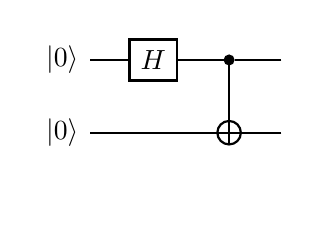
\begin{tikzpicture}
        \node[scale=1.0] {
            \begin{quantikz}
                \lstick{$\ket{0}$} & \gate{H} & \ctrl{1} & \qw \\
                \lstick{$\ket{0}$} & \qw      & \targ{}  & \qw \\
            \end{quantikz}
        };
    \end{tikzpicture}
    \caption{Circuit to prepare the first Bell state}
    \label{fig:bell00}
\end{figure}

\lstinputlisting[language=QHaskell,float,label=lst:bell,lastline=9,caption=Generating Bell state]{bell00.qh}

\cref{lst:bell} shows a circuit that corresponds to a suspended quantum computation that can be composed with other circuits. It takes no input and returns two qubits as output. The specification of the program is in its type (the first three lines). Here we see our first two propositions: the top predicate, $\top$, that is satisfied by any state space and the $X =_q \psi$ predicate that is satisfied by quantum variables, $X$, that lie in the span of the given state $\psi$. Intuitively, this circuit does not require any inputs and can work in any given state space and produces two qubits that are maximally entangled in the first Bell state $\ket{\beta_{00}}$.

\cref{lst:bella} shows how we can prove whether this program conforms to the given specification. The initialization command (at lines 6 and 10) allocates a new qubit, initialize it to $\ket{0}$ and binds it to the variable on the left side of $\leftarrow$. The strongest postcondition for unitary application simply involves applying the operator on the subspace specified by the precondition (on lines 9 and 13). Note that we use the $\Rightarrow$ symbol in these annotations for a simplification step, but it is not part of our predicate language.

\lstinputlisting[language=QHaskell,float,label=lst:bella,firstline=11,caption=Bell state program annotated with propositions]{bell00.qh}

\subsubsection{Quantum teleportation}
\label{sec:teleport}
Our second example shows how we can compose circuits defined in QHTT together and still maintain correctness. \Cref{fig:teleport} shows the circuit for quantum teleportation and the corresponding code is shown in \cref{lst:tele}. This example demonstrates how we can bind ghost variables in the Hoare type: $\{\psi: \mathit{vector}\}$ states that $\psi$ is a ghost variable of \textit{vector} type. Recall that ghost variables can only be used in the logical propositions and are not part of the program. We place the context declaring the ghost variables right after the output type to signal that the ghost variables are only bound in the \textit{require} and \textit{ensures} constructors that follow next in the Hoare type. We see another predicate $\mathbf{class}(q)$ here that states that the given qubit $q$ is in a classical state which is what we expect during quantum teleportation protocol. Or there would be no way to tell from the specification whether the implementation just returned the input qubit as the output!

\begin{figure}
    \centering
    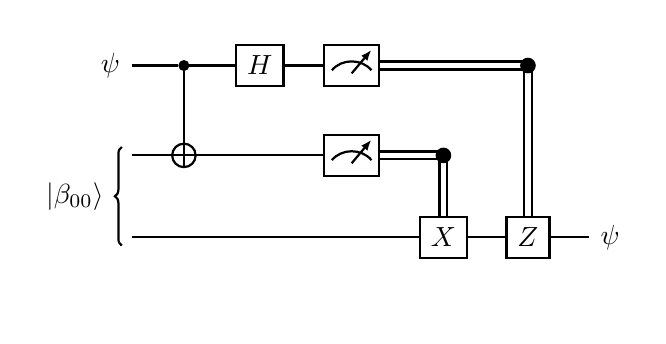
\begin{tikzpicture}
        \node[scale=1.0] {
            \begin{quantikz}
                \lstick{$\psi$}                & \ctrl{1} & \gate{H} & \meter{} & \cw        & \cwbend{2} \\
                \lstick[wires=2]{$\ket{\beta_{00}}$} & \targ{}  & \qw      & \meter{} & \cwbend{1} \\
						       \qw      & \qw      & \qw      & \qw        & \gate{X}   & \gate{Z} & \qw \rstick{$\psi$}\\
            \end{quantikz}
        };
    \end{tikzpicture}
    \caption{Quantum teleportation circuit}
    \label{fig:teleport}
\end{figure}

\lstinputlisting[language=QHaskell,float,label=lst:tele,lastline=13,caption=Quantum teleportation]{teleport.qh}

\lstinputlisting[language=QHaskell,float,label=lst:telea,firstline=15,caption=Annotated quantum teleportation program]{teleport.qh}

Verification steps for this program are shown in \cref{lst:telea}. At line 19, something interesting happens! When we measure a quantum variable (in the default computational basis), its state is collapsed to either classical bits 0 or 1 based on the distribution of either outcomes. In our logic, however, both the outcome and the distribution are still maintained. This is achieved by replacing the measured qubit (which is implicitly discarded with the measurement operation) in the state space under consideration with a ghost variable. If the quantum variable was previously entangled, it is replaced with a entangled ghost ($e$) and if it was unentangled with an unentangled ghost ($u$). Further, we maintain the correspondence between the classical bit that stores the measurement result and the ghost variable that replaced its corresponding qubit. So at line 21, $e_x$ corresponds to the classical bit $x$. Similarly, in lines 24-26, $e_y$ is introduced corresponding to $y$. This helps us in the next two steps of the program where operations controlled on the previous measurement outcomes are applied. We recover the original state $\psi$ at the end. Note that we use the comma symbol interchangeably with the conjunction symbol in the propositions.

This version of teleportation may not seem very interesting because it is essentially equivalent to teleportation performed without measurement (using the principle of deferred measurements). Hence, we turn out a more realistic variant in our next example.

\subsubsection{Modular teleportation with classical control}

As the teleportation protocol is usually stated, we have two agents Alice and Bob who share an entangled Bell pair at the beginning of the protocol. Alice wants to communicate a message encoded in a qubit to Bob. Alice performs a Bell measurement on her two qubits, the one that encodes the message and the other which is part of the entangled Bell pair. Then she sends the result of this measurement, two bits, to Bob. Bob receives those bits and performs correction steps on his qubit to obtain the message. We naturally can split the teleportation circuit into three parts: Bell state preparation, Alice's portion of the circuit and Bob's portion of the circuit.

\cref{lst:alice,lst:bob,lst:mtele} show the implementation of these parts in the form of separate modules (functions) along with their specifications as types. Alice's circuit requires that her second input qubit is entangled in the Bell state. This statement shows our first example of using Unruh's entangled ghost variable, $e$, in our specifications which is declared in the context right before the \textit{requires} construct along with other ghost variables. It further ensures that her two input qubits are both consumed in the process as they are asserted to be classical in the postcondition. Since Alice is dealing with entanglement, it is important to maintain the distribution over the all qubits involved including the ghost qubit $e$ and the newly created ghosts $e_x$ and $e_y$ because of her measurement operations.

Bob's specification shows what correction is applied if his qubit is in an arbitrary state. Note that Bob uses the classical control construct if-then-else in this variant of the circuit. The specification for teleport is the same as before but the implementation is now much shorter.

We show the annotated verification steps in \cref{lst:alicea,lst:boba,lst:mtelea}.

\lstinputlisting[language=QHaskell,float,label=lst:alice,caption=Alice's portion of teleportation,lastline=14]{teleport2.qh}

\lstinputlisting[language=QHaskell,float,label=lst:bob,caption=Bob's portion of teleportation,firstline=45,lastline=55]{teleport2.qh}

\lstinputlisting[language=QHaskell,float,label=lst:mtele,caption=Modular teleportation,firstline=74,lastline=82]{teleport2.qh}

\lstinputlisting[language=QHaskell,float,label=lst:alicea,caption=Annotated code for alice,firstline=16,lastline=43]{teleport2.qh}

\lstinputlisting[language=QHaskell,float,label=lst:boba,caption=Annotated code for bob,firstline=57,lastline=72]{teleport2.qh}

\lstinputlisting[language=QHaskell,float,label=lst:mtelea,caption=Annotated code for modular teleportation,firstline=84]{teleport2.qh}

% \subsubsection{Fair coin toss}

% \cref{lst:toss} shows a program along with its verification steps which produces a uniformly random bit. In this program we see the use of an unentangled ghost variable, $u_x$, at line 11 that records the outcome distribution of the measured qubit whose result is stored in the classical bit $x$.

% \lstinputlisting[language=QHaskell,float,label=lst:toss,firstline=10,caption=Fair coin toss]{cointoss.qh}

\subsubsection{Deutsch's algorithm}
\cref{lst:deutsch} demonstrates that our system can work in a higher-order setting where we can pass a circuit as input to another circuit and reason about the resulting computation. Here $U_f$ is a quantum oracle whose implementation is unknown but its type specifies everything we know about it --- it is parametrized over a classical function, $f$, that takes a bit and returns a bit; it takes two qubits as input and returns two qubits as output; and finally, if the input qubits store classical bits $x$ and $y$, then the output qubits store $x$ and $y \oplus f(x)$. The circuit $U_f$ is used as a blackbox in the implementation of Deutsch's algorithm as shown in \cref{fig:deutsch}. The idea is to be able to reason about the algorithm's correctness using the type of the blackbox alone.
% This example involves various propositions about classical bits that we did not describe, but it serves to show that if our predicate language is extended with standard classical logic (ie, predicates such as equality of classical bits, $=_c$ and implication, $=>$) we can say a lot more in the specification.

\begin{figure}
    \centering
    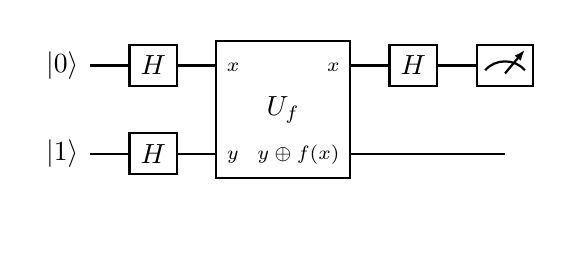
\begin{tikzpicture}
        \node[scale=1.0] {
            \begin{quantikz}
                \lstick{$\ket{0}$} & \gate{H} & \gate[wires=2][1.7cm]{U_f}\gateinput{$x$}
                \gateoutput{$x$} & \gate{H} & \meter{} \\
                \lstick{$\ket{1}$} & \gate{H} & \gateinput{$y$}\gateoutput{$y\oplus f(x)$} & \qw & \qw \\
            \end{quantikz}
        };
    \end{tikzpicture}
    \caption{Quantum circuit for Deutsch's algorithm}
    \label{fig:deutsch}
\end{figure}

\lstinputlisting[language=QHaskell,float,label=lst:deutsch,caption=Deutsch's algorithm]{deutsch.qh}

\section{Discussion and related work}

In \cref{sec:teleport}, when we presented code for quantum teleportation, it was apparent from its type (or specification) that the quantum variables $q$ (input) and $b$ (output) are different because of the proposition $\mathbf{class}(q)$ which suggests that $q$ is discarded in the postcondition. It would be nicer if we could also specify information about the resource usage of the program; in teleportation, for example, an EPR pair gets consumed along with the input qubit.

TODO:

- compare with existing hoare logics

\subsection{Verification of Quantum Programs}
Previous work, such as Proto-Quipper~\cite{rios2017,rios2017} and QWire~\cite{qwire2017,qwirepractice2017,rand2018} utilize a linear type system and dependent types to enforce a small subset of semantic properties, such as the no-cloning restriction and whether a unitary gate is of the right dimension. These advances in quantum type systems, although helpful, still fall short in encoding and enforcing even more useful properties that one would like to be able to express for the purpose of verification.

Our approach builds upon previous work in reasoning about quantum programs such as Quantum Weakest Preconditions~\cite{dhondt2006} and Quantum Hoare Logic~\cite{floydhoare2012} in the spirit of \cite{hoare1969} and \cite{dijkstra1976} but attempts to bring those reasoning techniques into the type system. The hope is that programmers will be able to encode some of the semantic properties that they expect of their programs as specifications in their code and type checking will ensure correctness of some of those properties. In the classical setting, Hoare Type Theory (HTT)~\cite{nanevski2008} accomplishes exactly this goal. Our attempt is to merge these ideas for the quantum realm.

\section{Conclusion and perspectives}
\label{sec:conclusion}
In this paper, we described our work on Quantum Hoare Type Theory which is a dependently typed functional programming language with support for quantum computation. We used the novel quantum Hoare logic by Unruh~\cite{unruh2019} that helped us compactly specify properties about quantum state. We further demonstrated the usefulness of our approach using basic examples including bell state preparation and quantum teleportation.

With future work on code extraction, our approach can become a unified system for programming, specification, and reasoning about quantum computation.

There are several other avenues to explore:

\paragraph{Quantum Language} Our programming language currently does not support any iterative or recursive constructs. We would like to add those in future. Further, currently it is not possible to construct pure unitary operators directly in our language apart from those provided as constants. As \cite{qio} show, unitary operations form an algebraic monoidal structure and it will be really nice to be able construct arbitrary unitaries in the language which will greatly enhance its expressive power from current Clifford circuits to a universal language.

\paragraph{Mechanization} There are multiple implementations of HTT in Coq such as Ynot~\cite{ynot2008}. We would like to mechanize QHTT in Coq, F* or some such dependent type theory for higher assurance of the usefulness and soundness of QHTT. This will also enable us to extract verified circuits in a lower level quantum language such as OpenQASM~\cite{cross2017} for execution on real machines.

\paragraph{Linearity} Peter Selinger and collaborators have recently proposed a linear dependent typed version of Proto-Quipper (dubbed Proto-Quipper-D)~\cite{selinger2020,fu2020linear}. It is an interesting challenge to reconcile linearity in our theory based on their proposal.

\paragraph{Circuits as Arrows} Further, Proto-Quipper treats quantum circuits as first class citizens of the language. We would like to explore modifying our theory to treat Quantum Hoare types as arrows instead of as monads as was suggested by \cite{so-arrows}. It makes sense from the perspective of sequential composition as arrows can have an arbitrary number of input/outputs as opposed to monads.

\paragraph{Behavioural Types} Another venue for exploration is to incorporate more precise types for qubits that can distinguish between qubits in pure classical state vs. those in superposition vs. those in entanglement~\cite{JorrandPerdrix2009} such as those inspired by the various quantum resource theories or the Heisenberg representation of quantum mechanics~\cite{rssl2019,rssl20}.

\paragraph{Classical Effects} Finally, it will be an interesting challenge to reconcile both classical and quantum effects together in a single theory of effects.

\section*{Acknowledgements}
I thank John Reppy, Robert Rand and the anonymous reviewers of QPL 2020 for their feedback on an earlier presentation of this work.

This material is based upon work supported by EPiQC, an NSF Expedition in Computing, under Grant No. 1730449. Any opinions, findings, and conclusions or recommendations expressed in this material are those
of the author and do not necessarily reflect the views of the National Science Foundation.

\bibliographystyle{eptcsalpha}
\bibliography{references}

\appendix

\section{Grammar}

\nonterms{Typ}
\nonterms{MonoTyp}
\nonterms{Prop}
\nonterms{Tm}
\nonterms{Cmd}
\nonterms{Unitary}
\nonterms{Comp}
\nonterms{Ctx}

\section{Inference rules}

\subsection{Valid contexts}

\drules[ctx]{$\vdash \Gamma$ \textbf{ctx}}{context formation}{Empty,Type,Prop}

\subsection{Valid types}

\drules[ty]{$\Gamma \vdash A$ \textbf{type}}{type formation}{Unit,Bit,Qbit,Prop,Pi,Pair,Hoare}

\subsection{Terms}

\drules[tm]{$\Gamma \vdash M : A$}{term typing}{VarE,UnitI,ZeroI,OneI,VectorI,PiI,PiE,PairI,FstE,SndE,AscriptionE}

\subsection{Well-formed propositions}

\drules[prop]{$\Gamma \vdash P : prop$}{checking propositions}{TopI,BotI,ConjI,DisjI,UnI}

% \subsection{Trivial examples}

% \lstinputlisting[language=QHaskell,caption=Several simple examples from Q\# Quantum Katas]{qsharp.qh}

\end{document}
